\documentclass[11pt,a4paper,]{article}
\usepackage{lmodern}

\usepackage{amssymb,amsmath}
\usepackage{ifxetex,ifluatex}
\usepackage{fixltx2e} % provides \textsubscript
\ifnum 0\ifxetex 1\fi\ifluatex 1\fi=0 % if pdftex
  \usepackage[T1]{fontenc}
  \usepackage[utf8]{inputenc}
\else % if luatex or xelatex
  \usepackage{unicode-math}
  \defaultfontfeatures{Ligatures=TeX,Scale=MatchLowercase}
\fi
% use upquote if available, for straight quotes in verbatim environments
\IfFileExists{upquote.sty}{\usepackage{upquote}}{}
% use microtype if available
\IfFileExists{microtype.sty}{%
\usepackage[]{microtype}
\UseMicrotypeSet[protrusion]{basicmath} % disable protrusion for tt fonts
}{}
\PassOptionsToPackage{hyphens}{url} % url is loaded by hyperref
\usepackage[unicode=true]{hyperref}
\hypersetup{
            pdftitle={A fast and elegant method for forecast reconciliation using linear forecasting models},
            pdfkeywords={hierarchical forecasting, grouped forecasting, reconciling forecast, linear regression},
            pdfborder={0 0 0},
            breaklinks=true}
\urlstyle{same}  % don't use monospace font for urls
\usepackage{geometry}
\geometry{left=2.5cm,right=2.5cm,top=2.5cm,bottom=2.5cm}
\usepackage[style=authoryear-comp,]{biblatex}
\addbibresource{references.bib}
\usepackage{longtable,booktabs}
% Fix footnotes in tables (requires footnote package)
\IfFileExists{footnote.sty}{\usepackage{footnote}\makesavenoteenv{long table}}{}
\IfFileExists{parskip.sty}{%
\usepackage{parskip}
}{% else
\setlength{\parindent}{0pt}
\setlength{\parskip}{6pt plus 2pt minus 1pt}
}
\setlength{\emergencystretch}{3em}  % prevent overfull lines
\providecommand{\tightlist}{%
  \setlength{\itemsep}{0pt}\setlength{\parskip}{0pt}}
\setcounter{secnumdepth}{5}

% set default figure placement to htbp
\makeatletter
\def\fps@figure{htbp}
\makeatother


\title{A fast and elegant method for forecast reconciliation using linear forecasting models}

%% MONASH STUFF

%% CAPTIONS
\RequirePackage{caption}
\DeclareCaptionStyle{italic}[justification=centering]
 {labelfont={bf},textfont={it},labelsep=colon}
\captionsetup[figure]{style=italic,format=hang,singlelinecheck=true}
\captionsetup[table]{style=italic,format=hang,singlelinecheck=true}

%% FONT
\RequirePackage{bera}
\RequirePackage{mathpazo}

%% HEADERS AND FOOTERS
\RequirePackage{fancyhdr}
\pagestyle{fancy}
\rfoot{\Large\sffamily\raisebox{-0.1cm}{\textbf{\thepage}}}
\makeatletter
\lhead{\textsf{\expandafter{\@title}}}
\makeatother
\rhead{}
\cfoot{}
\setlength{\headheight}{15pt}
\renewcommand{\headrulewidth}{0.4pt}
\renewcommand{\footrulewidth}{0.4pt}
\fancypagestyle{plain}{%
\fancyhf{} % clear all header and footer fields
\fancyfoot[C]{\sffamily\thepage} % except the center
\renewcommand{\headrulewidth}{0pt}
\renewcommand{\footrulewidth}{0pt}}

%% MATHS
\RequirePackage{bm,amsmath}
\allowdisplaybreaks

%% GRAPHICS
\RequirePackage{graphicx}
\setcounter{topnumber}{2}
\setcounter{bottomnumber}{2}
\setcounter{totalnumber}{4}
\renewcommand{\topfraction}{0.85}
\renewcommand{\bottomfraction}{0.85}
\renewcommand{\textfraction}{0.15}
\renewcommand{\floatpagefraction}{0.8}

%\RequirePackage[section]{placeins}

%% SECTION TITLES
\RequirePackage[compact,sf,bf]{titlesec}
\titleformat{\section}[block]
  {\fontsize{15}{17}\bfseries\sffamily}
  {\thesection}
  {0.4em}{}
\titleformat{\subsection}[block]
  {\fontsize{12}{14}\bfseries\sffamily}
  {\thesubsection}
  {0.4em}{}
\titlespacing{\section}{0pt}{*5}{*1}
\titlespacing{\subsection}{0pt}{*2}{*0.2}


%% TITLE PAGE
\def\Date{\number\day}
\def\Month{\ifcase\month\or
 January\or February\or March\or April\or May\or June\or
 July\or August\or September\or October\or November\or December\fi}
\def\Year{\number\year}

\makeatletter
\def\wp#1{\gdef\@wp{#1}}\def\@wp{??/??}
\def\jel#1{\gdef\@jel{#1}}\def\@jel{??}
\def\showjel{{\large\textsf{\textbf{JEL classification:}}~\@jel}}
\def\nojel{\def\showjel{}}
\def\addresses#1{\gdef\@addresses{#1}}\def\@addresses{??}
\def\cover{{\sffamily\setcounter{page}{0}
        \thispagestyle{empty}
        \placefig{2}{1.5}{width=5cm}{monash2}
        \placefig{16.9}{1.5}{width=2.1cm}{MBusSchool}
        \begin{textblock}{4}(16.9,4)ISSN 1440-771X\end{textblock}
        \begin{textblock}{7}(12.7,27.9)\hfill
        
\includegraphics[height=0.7cm]{AACSB}~~~
        
\includegraphics[height=0.7cm]{EQUIS}~~~
        
\includegraphics[height=0.7cm]{AMBA}
        \end{textblock}
        \vspace*{2cm}
        \begin{center}\Large
        Department of Econometrics and Business Statistics\\[.5cm]
        \footnotesize http://monash.edu/business/ebs/research/publications
        \end{center}\vspace{2cm}
        \begin{center}
        \fbox{\parbox{14cm}{\begin{onehalfspace}\centering\Huge\vspace*{0.3cm}
                \textsf{\textbf{\expandafter{\@title}}}\vspace{1cm}\par
                \LARGE\@author\end{onehalfspace}
        }}
        \end{center}
        \vfill
                \begin{center}\Large
                \Month~\Year\\[1cm]
                Working Paper \@wp
        \end{center}\vspace*{2cm}}}
\def\pageone{{\sffamily\setstretch{1}%
        \thispagestyle{empty}%
        \vbox to \textheight{%
        \raggedright\baselineskip=1.2cm
     {\fontsize{24.88}{30}\sffamily\textbf{\expandafter{\@title}}}
        \vspace{2cm}\par
        \hspace{1cm}\parbox{14cm}{\sffamily\large\@addresses}\vspace{1cm}\vfill
        \hspace{1cm}{\large\Date~\Month~\Year}\\[1cm]
        \hspace{1cm}\showjel\vss}}}
\def\blindtitle{{\sffamily
     \thispagestyle{plain}\raggedright\baselineskip=1.2cm
     {\fontsize{24.88}{30}\sffamily\textbf{\expandafter{\@title}}}\vspace{1cm}\par
        }}
\def\titlepage{{\cover\newpage\pageone\newpage\blindtitle}}

\def\blind{\def\titlepage{{\blindtitle}}\let\maketitle\blindtitle}
\def\titlepageonly{\def\titlepage{{\pageone\end{document}}}}
\def\nocover{\def\titlepage{{\pageone\newpage\blindtitle}}\let\maketitle\titlepage}
\let\maketitle\titlepage
\makeatother

%% SPACING
\RequirePackage{setspace}
\spacing{1.5}

%% LINE AND PAGE BREAKING
\sloppy
\clubpenalty = 10000
\widowpenalty = 10000
\brokenpenalty = 10000
\RequirePackage{microtype}

%% PARAGRAPH BREAKS
\setlength{\parskip}{1.4ex}
\setlength{\parindent}{0em}

%% HYPERLINKS
\RequirePackage{xcolor} % Needed for links
\definecolor{darkblue}{rgb}{0,0,.6}
\RequirePackage{url}

\makeatletter
\@ifpackageloaded{hyperref}{}{\RequirePackage{hyperref}}
\makeatother
\hypersetup{
     citecolor=0 0 0,
     breaklinks=true,
     bookmarksopen=true,
     bookmarksnumbered=true,
     linkcolor=darkblue,
     urlcolor=blue,
     citecolor=darkblue,
     colorlinks=true}

%% KEYWORDS
\newenvironment{keywords}{\par\vspace{0.5cm}\noindent{\sffamily\textbf{Keywords:}}}{\vspace{0.25cm}\par\hrule\vspace{0.5cm}\par}

%% ABSTRACT
\renewenvironment{abstract}{\begin{minipage}{\textwidth}\parskip=1.4ex\noindent
\hrule\vspace{0.1cm}\par{\sffamily\textbf{\abstractname}}\newline}
  {\end{minipage}}


\usepackage[T1]{fontenc}
\usepackage[utf8]{inputenc}

\usepackage[showonlyrefs]{mathtools}
\usepackage[no-weekday]{eukdate}

%% BIBLIOGRAPHY

\makeatletter
\@ifpackageloaded{biblatex}{}{\usepackage[style=authoryear-comp, backend=biber, natbib=true]{biblatex}}
\makeatother
\ExecuteBibliographyOptions{bibencoding=utf8,minnames=1,maxnames=3, maxbibnames=99,dashed=false,terseinits=true,giveninits=true,uniquename=false,uniquelist=false,doi=false, isbn=false,url=true,sortcites=false}

\DeclareFieldFormat{url}{\texttt{\url{#1}}}
\DeclareFieldFormat[article]{pages}{#1}
\DeclareFieldFormat[inproceedings]{pages}{\lowercase{pp.}#1}
\DeclareFieldFormat[incollection]{pages}{\lowercase{pp.}#1}
\DeclareFieldFormat[article]{volume}{\mkbibbold{#1}}
\DeclareFieldFormat[article]{number}{\mkbibparens{#1}}
\DeclareFieldFormat[article]{title}{\MakeCapital{#1}}
\DeclareFieldFormat[inproceedings]{title}{#1}
\DeclareFieldFormat{shorthandwidth}{#1}
% No dot before number of articles
\usepackage{xpatch}
\xpatchbibmacro{volume+number+eid}{\setunit*{\adddot}}{}{}{}
% Remove In: for an article.
\renewbibmacro{in:}{%
  \ifentrytype{article}{}{%
  \printtext{\bibstring{in}\intitlepunct}}}

\makeatletter
\DeclareDelimFormat[cbx@textcite]{nameyeardelim}{\addspace}
\makeatother
\renewcommand*{\finalnamedelim}{%
  %\ifnumgreater{\value{liststop}}{2}{\finalandcomma}{}% there really should be no funny Oxford comma business here
  \addspace\&\space}


\wp{no/yr}
\jel{C10,C14,C22}

\RequirePackage[absolute,overlay]{textpos}
\setlength{\TPHorizModule}{1cm}
\setlength{\TPVertModule}{1cm}
\def\placefig#1#2#3#4{\begin{textblock}{.1}(#1,#2)\rlap{\includegraphics[#3]{#4}}\end{textblock}}


\nocover

\author{Mahsa~Ashouri, Rob J~Hyndman, Galit~Shmueli}
\addresses{\textbf{Mahsa Ashouri}\newline
Institute of Service Science, National Tsing Hua University, Taiwan
\newline{Email: \href{mailto:mahsa.ashouri@iss.nthu.edu.tw}{\nolinkurl{mahsa.ashouri@iss.nthu.edu.tw}}}\newline Corresponding author\\[1cm]
\textbf{Rob J Hyndman}\newline
Monash University, Clayton VIC 3800, Australia
\newline{Email: \href{mailto:rob.hyndman@monash.edu}{\nolinkurl{rob.hyndman@monash.edu}}}\\[1cm]
\textbf{Galit Shmueli}\newline
Institute of Service Science, National Tsing Hua University, Taiwan
\newline{Email: \href{mailto:galit.shmueli@iss.nthu.edu.tw}{\nolinkurl{galit.shmueli@iss.nthu.edu.tw}}}\\[1cm]
}

\date{\sf\Date~\Month~\Year}
\makeatletter
 \lfoot{\sf Ashouri, Hyndman, Shmueli: \@date}
\makeatother

%% Any special functions or other packages can be loaded here.

\usepackage{booktabs}
\usepackage{float}
\usepackage{longtable}
\usepackage{cases}
\usepackage{array}
\usepackage{todonotes}
%\usepackage[backend=biber]{biblatex}
%\usepackage[backend=biber, bibencoding=utf8, style=authoryear, citestyle=authoryear]{biblatex}

\mathtoolsset{showonlyrefs=true}
\allowdisplaybreaks

\usepackage{float}
\floatplacement{figure}{!htbp}

\def\addlinespace{}
\usepackage[section]{placeins}


\begin{document}
\maketitle
\begin{abstract}
Forecasting hierarchical or grouped time series involves two steps: computing base forecasts and reconciling the forecasts. Base forecasts can be computed by popular time series forecasting methods such as Exponential Smoothing (ETS) and Autoregressive Integrated Moving Average (ARIMA) models. The reconciliation step is a linear process that adjusts the base forecasts to ensure they are coherent. However using ETS or ARIMA for base forecasts can be computationally challenging when there are a large number of series to forecast, as each model must be numerically optimized for each series. We propose a linear model that avoids this computational problem, and uses a single-step approach to obtain the forecasts, rather than the usual two-step approach. The proposed method is very flexible in incorporating external data and handling missing values. We illustrate our approach using two datasets: monthly Australian domestic tourism and daily Wikipedia pageviews. We compare our approach to reconciliation using ETS and ARIMA, and show that our approach is much faster while providing similar levels of forecast accuracy.
\end{abstract}
\begin{keywords}
hierarchical forecasting, grouped forecasting, reconciling forecast, linear regression
\end{keywords}

\hypertarget{introduction}{%
\section{Introduction}\label{introduction}}

Modern data collection tools have dramatically increased the amount of available time series data. For example, the Internet of Things and point-of-sale scanning produce huge volumes of time series in a short period of time. Naturally, there is an interest in forecasting these time series, yet forecasting large collections of time series is computationally challenging.

\hypertarget{hierarchical-and-grouped-time-series}{%
\subsection{Hierarchical and grouped time series}\label{hierarchical-and-grouped-time-series}}

In many cases, these time series can be structured and disaggregated based on hierarchies or groups such as geographic location, product type, gender, etc. An example of hierarchical time series is sales in restaurant chains, which can be disaggregated into different stores and then different types of food or drinks. Figure \ref{fig:hierarchicalexample} shows a schematic of such a hierarchical time series structure with three levels. The top level (level 0) is the total series, formed by aggregating all the bottom level series. In the middle level (level 1), series are aggregations of their own child series; for instance, series A is the aggregation of AA and AB. Finally, the bottom level series (level 2), includes the most disaggregated series.\todo{I suggest we label Level 2 with AW, AX, BY, BZ to avoid confusion.}

\begin{figure}

{\centering 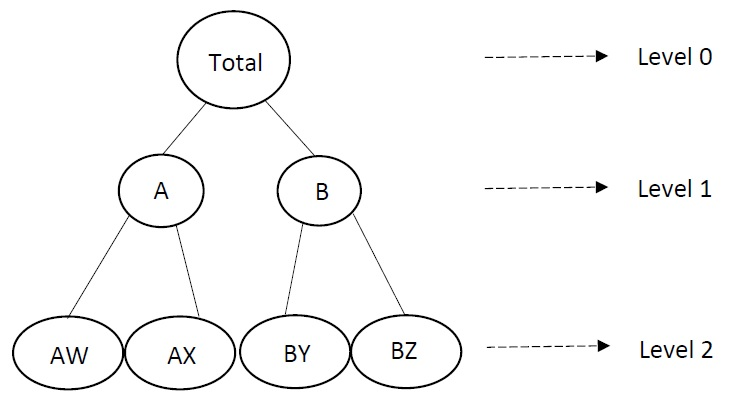
\includegraphics[width=280px,height=180px]{Paper-Figures/hierarchical_example} 

}

\caption{An example of a two level hierarchical structure}\label{fig:hierarchicalexample}
\end{figure}

Grouped time series involve more complicated aggregation structures compared to strictly hierarchical time series. To take the simplest example, suppose we have two grouping factors which are not nested: sex (Male/Female) and city (New York/San Francisco). The disaggregated series for each combination of sex and city can be combined to form city sub-totals, or sex sub-totals. These sub-totals can be combined to give the overall total. Both sub-totals are of interest.

We can think of such structures as hierarchical time series without a unique hierarchy. A schematic of this grouped time series structure is shown in Figure \ref{fig:groupexample} with two grouping factors, each of two levels (A/B and C/D). The series in this structure can be split first into groups A and B and then subdivided further into C and D (left side), or split first into C and D and then subdivided into A and B (right side). The final disaggregation is identical in both cases, but the middle level aggregates are different.

\begin{figure}

{\centering 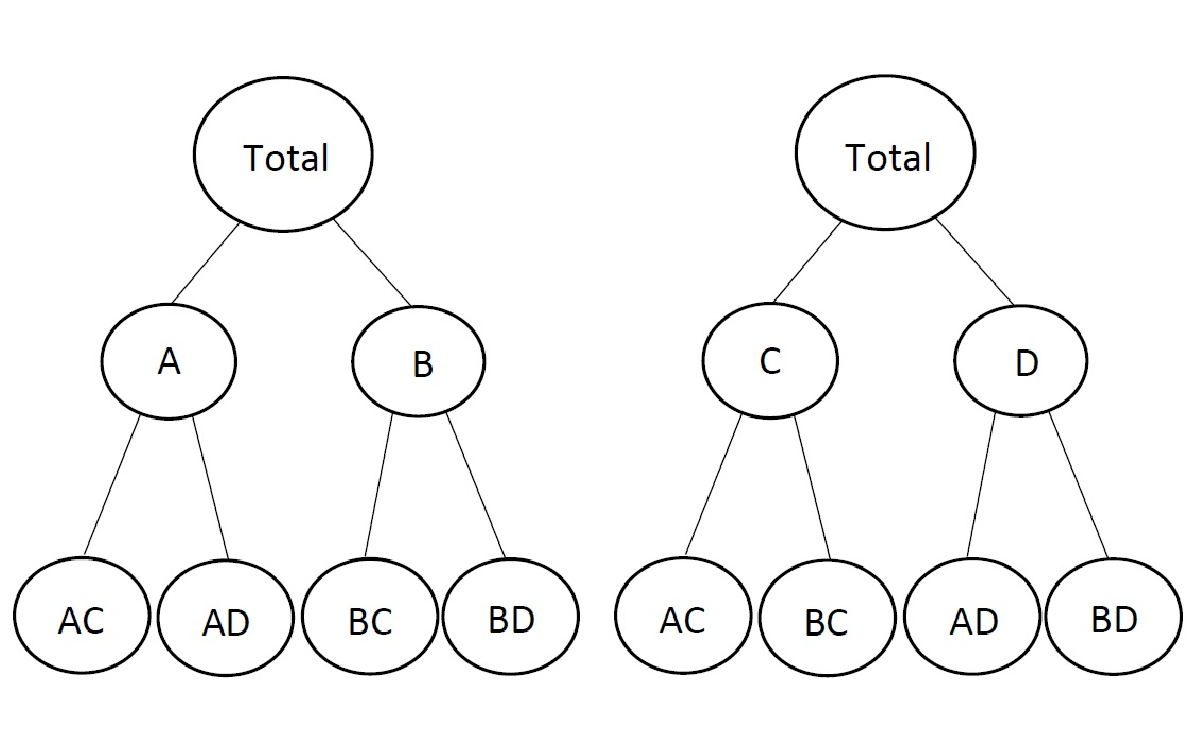
\includegraphics[width=330px,height=180px]{hcf_files/figure-latex/groupexample-1} 

}

\caption{An example of two level grouped structure}\label{fig:groupexample}
\end{figure}

We use the same notation \autocite[following][]{fpp2} for both hierarchical and grouped time series. We denote the total series at time \(t\) by \(y_t\), and the series at node \(Z\) and time \(t\) by \(y_{Z,t}\). For describing the relationships between series, we use an \(n\times m\) matrix, called the `summing matrix', denoted by \(\bm{S}\), in which \(n\) is the overall number of nodes and \(m\) is the number of bottom level nodes. For example in Figure \ref{fig:hierarchicalexample}, \(n = 7\) and \(m = 4\), while in Figure \ref{fig:groupexample}, \(n=9\) and \(m=4\). Then we can write \(\bm{y}_t=\bm{S}\bm{b}_t\), where \(\bm{y}_t\) is a vector of all the level nodes at time \(t\) and \(\bm{b}_t\) is the vector of all the bottom level nodes at time \(t\). For the example shown in Figure \ref{fig:groupexample}, the equation can be written as follows:
\begin{equation}\label{eq:Smatrixexample}
\begin{pmatrix}
  y_{t}\\y_{A,t}\\y_{B,t}\\y_{C,t}\\y_{D,t}\\y_{AC,t}\\y_{AD,t}\\y_{BC,t}\\y_{BD,t}
\end{pmatrix} =
\begin{pmatrix}
  1&1&1&1\\1&1&0&0\\0&0&1&1\\1&0&1&0\\0&1&0&1\\1&0&0&0\\0&1&0&0\\0&0&1&0\\0&0&0&1\\
\end{pmatrix}
\begin{pmatrix}
  y_{AC,t}\\y_{AD,t}\\y_{BC,t}\\y_{BD,t}\\
\end{pmatrix}.
\end{equation}

\hypertarget{forecasting-hierarchical-time-series}{%
\subsection{Forecasting hierarchical time series}\label{forecasting-hierarchical-time-series}}

If we just forecast each series individually, we are ignoring the hierarchical or grouping structure, and the forecasts will not be ``coherent'' (they will not add up appropriately).

There are several available methods that consider the hierarchical structure information when forecasting time series. These include the top-down \autocites{gross1990disaggregation}{fliedner2001hierarchical}, bottom-up \autocite{kahn1998revisiting}, middle-out and optimal combination \autocite{hyndman2011optimal} approaches. In the top-down approach, we first forecast the total series and then disaggregate the forecast to form lower level series forecasts based on a set of historical and forecasted proportions \autocite[for details see][]{athanasopoulos2009hierarchical}. In the bottom-up approach, the forecasts in each level of the hierarchy can be computed by aggregating the bottom level series forecasts. However, we may not get good upper-level forecasts because the most disaggregated series can be noisy and so their forecasts are often inaccurate. In the middle-out approach, the process can be started from one of the middle levels and other forecasts can be computed using aggregation for upper levels and disaggregation for lower levels. Finally, optimal combination uses all the \(n\) forecasts for all of the series in the entire structure, and then uses an optimization process to reconcile the resulting forecasts. The advantage of the optimal combination method, compared with the other methods, is that it considers all information in the hierarchy, including any correlations among the series.

In the optimal combination method, reconciled forecasts can be computed using \autocite{mint2018}
\begin{equation}\label{eq:mint}
  \tilde{\bm{y}}_{h}=\bm{S}(\bm{S}'\bm{W}_h^{-1}\bm{S})^{-1}\bm{S}'\bm{W}^{-1}\hat{\bm{y}}_h,
\end{equation}
where \(\hat{\bm{y}}_h\) represents a vector of \(h\)-step-ahead base forecasts for all levels of the hierarchy, and \(\bm{W}_h\) is the variance matrix of forecast errors for the \(h\)-step-ahead base forecasts.

The most difficult task is to compute \(\bm{W}_h\), but \textcite{mint2018} and \textcite{hyndman2016fast} argue that replacing it by the diagonal of \(\bm{W}_1\) gives good results in practice. This is easy to obtain because it is simply the diagonal matrix comprising the residual variances from each of the base forecasts.

The most computationally challenging part of the optimal combination method is to produce all the base forecasts that make up \(\hat{\bm{y}}_h\). In many applications, there may be thousands or even millions of individual series, and each of them must be forecast independently. The most popular time series forecasting methods such as ETS and ARIMA models \autocite{fpp2} involve non-linear optimization routines to estimate the parameters via maximum likelihood estimation. Usually, multiple models are fitted for each series, and the best is select by minimizing Akaike's Information Citerion \autocite{akaike1998information}. This computational challenges increases with the number of lower level series as well as in the number of aggregations of interest.

We therefore propose a new approach to compute the base forecasts that is both computationally fast while maintaining an acceptable forecasting accuracy level.

\hypertarget{proposed-approach}{%
\section{Proposed approach}\label{proposed-approach}}

Our proposed approach is based on using linear regression models for computing base forecasts. Suppose we have a linear model that we use for forecasting, and we wish to apply it to \(N\) different series which have some aggregation constraints. We have observations \(y_{t,i}\) from times \(t=1,\dots,T\) and series \(i=1,\dots,N\). Then
\begin{equation}
y_{t,i} = \bm{\beta}_{i}' \bm{x}_{t,i} + \varepsilon_{t,i}
\end{equation}
where \(\bm{x}_{t,i}=\{1, x_{t,i,1},\dots,x_{t,i,p}\}\) is a \((p+1)\)-vector of regression variables, and \(\varepsilon_{t,i}\sim \text{NID}(0,\sigma_i^2)\). This equation for all the observations in matrix form can be written as follows:
\begin{equation}\label{eq:linearmodel}
\begin{pmatrix}
\bm{y}_1\\
\bm{y}_2\\
\bm{y}_3 \\
\vdots\\
\bm{y}_N
\end{pmatrix}=
\begin{pmatrix}
\bm{X}_1 & 0        & 0       & \dots  & 0\\
0        & \bm{X}_2 & 0        & \dots  & 0\\
0        & 0        & \bm{X}_3 & \ddots & \vdots \\
\vdots   & \vdots   & \ddots   & \ddots & 0\\
0        & 0    & \dots    & 0      & \bm{X}_N
\end{pmatrix}
\begin{pmatrix}
\bm{\beta}_1\\
\bm{\beta}_2\\
\bm{\beta}_3\\
\vdots\\
\bm{\beta}_N
\end{pmatrix}+
\begin{pmatrix}
\bm{\varepsilon}_1\\
\bm{\varepsilon}_2\\
\bm{\varepsilon}_3\\
\vdots \\
\bm{\varepsilon}_N
\end{pmatrix},
\end{equation}
where \(\bm{y}_i = \{y_{1,i}, y_{2,i}, \dots, y_{T,i}\}\) is a \(T\)-vector, \({\bm{\beta}}_i = \{\beta_{0,i}, \beta_{1,i}, \beta_{2,i}, \dots, \beta_{p,i}\}\) is a \((p+1)\)-vector, \({\bm{\varepsilon}}_i = \{\varepsilon_{1,i}, \varepsilon_{2,i}, \dots, \varepsilon_{T,i}\}\) is a \(T\)-vector and \(\bm{X}_i\) is the \(T\times (p+1)\)-matrix
\begin{equation}
\bm{X}_i = \begin{pmatrix}
1 & x_{1,i,1} & x_{1,i,2} & \dots & x_{1,i,p}\\
1 & x_{2,i,1} & x_{2,i,2} & \dots & x_{2,i,p}\\
\vdots & \vdots & \vdots & & \vdots \\
1 & x_{T,i,1} & x_{T,i,2} & \dots & x_{T,i,p}\\
\end{pmatrix}.
\end{equation}

Equation \eqref{eq:linearmodel} can be written as \(\bm{Y} = \bm{X} \bm{B} + \bm{E}\), with parameter estimates given by \(\hat{\bm{B}} = (\bm{X}'\bm{X})^{-1} \bm{X}'\bm{Y}\). Then the base forecasts are obtained using
\begin{equation}\label{eq:baseforecats}
\hat{\bm{y}}_{t+h} = \bm{X}_{t+h}^* \hat{\bm{B}},
\end{equation}
where \(\hat{\bm{y}}_{t+h}\) is an \(N\)-vector of forecasts, \(\hat{\bm{B}}\) comprises \(N\) stacked \((p+1)\)-vectors of estimated coefficients, and \(\bm{X}_{t+h}^*\) is the \(N\times N(p+1)\) matrix
\pagebreak[3]\begin{equation}
\bm{X}_{t+h}^* =
\begin{pmatrix}
\bm{x}_{t+h,1}' & 0                & 0                & \dots  & 0\\
0               & \bm{x}_{t+h,2}' & 0                & \dots  & 0\\
0               & 0                & \bm{x}_{t+h,3}' & \ddots & \vdots \\
\vdots          & \vdots           & \ddots           & \ddots & 0\\
0               & 0                & \dots            & 0      & \bm{x}_{t+h,N}'
\end{pmatrix}.
\end{equation}
Note that we use \(\bm{X}^*_{t}\) to distinguish this matrix, which combines \(\bm{x}_{t,i}\) across all series for one time from \(\bm{X}_i\) which combines \(\bm{x}_{t,i}\) across all time for one series.

The reconciliation (of the WLS variety), using Equation \eqref{eq:mint} can be written as
\begin{equation}\label{eq:recforecasts}
\tilde{\bm{y}}_{t+h} = (\bm{S}'\bm{W}\bm{S})^{-1}\bm{S}'\bm{W}\hat{\bm{y}}_{t+h},
\end{equation}
where \(\bm{W}\) is an \(N\times N\) diagonal matrix with \((i,i)\)th element \(\sigma_i^2\), and \(\bm{S}\) is the summation matrix containing the aggregation constraints.

Finally, we can combine the two linear equations for computing base forecasts and reconciled forecasts (Equations \eqref{eq:baseforecats} and \eqref{eq:recforecasts}) to obtain the reconciled forecasts with a single equation:
\begin{equation}\label{eq:singlestep}
\tilde{\bm{y}}_{t+h} = (\bm{S}'\bm{W}\bm{S})^{-1}\bm{S}'\bm{W}
                        (\bm{X}_{t+h}^* \hat{\bm{B}})
                        = (\bm{S}'\bm{W}\bm{S})^{-1}\bm{S}'\bm{W}
                        (\bm{X}_{t+h}^* \bm{X}'\bm{X})^{-1} \bm{X}'\bm{Y}.
\end{equation}

\hypertarget{proposed-approach-with-same-set-of-bmx}{%
\subsection{\texorpdfstring{Proposed approach with same set of \(\bm{X}\)}{Proposed approach with same set of \textbackslash{}bm\{X\}}}\label{proposed-approach-with-same-set-of-bmx}}

If we have same set of regression variables, \(\bm{X}\), for all the series, we can write the above equations more easily using multivariate regression equations, and we can obtain all the reconciled forecasts for all the series in one equation. In that case Equation \eqref{eq:linearmodel} can be rearranged as follows:
\begin{equation}\label{eq:linearmodelsameX}
  \begin{pmatrix}
  y_{11} & \dots & y_{1N}\\
  y_{21} & \dots & y_{2N}\\
  \vdots &       & \vdots\\
  y_{T1} & \dots & y_{TN}
  \end{pmatrix} =
  \begin{pmatrix}
  1      & X_{11} & \dots & X_{1p}\\
  1      & X_{21} & \dots & X_{2p}\\
  \vdots & \vdots &       & \vdots\\
  1      & X_{T1} & \dots & X_{Tp}
  \end{pmatrix}
  \begin{pmatrix}
  \beta_{01} & \dots & \beta_{0N}\\
  \beta_{11} & \dots & \beta_{1N}\\
  \vdots     &       & \vdots\\
  \beta_{p1} & \dots & \beta_{pN}
  \end{pmatrix} \\
  +
  \begin{pmatrix}
  \varepsilon_{11} & \dots & \varepsilon_{1N}\\
  \varepsilon_{21} & \dots & \varepsilon_{2N}\\
  \vdots           &       & \vdots\\
  \varepsilon_{T1} & \dots & \varepsilon_{TN}
  \end{pmatrix}
\end{equation}

We can represent Equation \eqref{eq:linearmodelsameX} as follows
\begin{equation}\label{eq:linearmodelmatrixsameX}
\bm{Y}= \bm{X} \bm{B} + \bm{E},
\end{equation}
where \(\bm{Y}\), \(\bm{X}\), \(\bm{B}\) and \(\bm{E}\) are now matrices of size \(T\times N\), \(T\times (p+1)\), \((p+1)\times N\) and \(T \times N\), respectively. Using Equation \eqref{eq:linearmodelmatrixsameX}, parameter estimates are given by
\begin{equation}
\hat{\bm{B}} = (\bm{X}'\bm{X})^{-1} \bm{X}'\bm{Y}.
\end{equation}
Then the base forecasts can be written as
\begin{equation}
\begin{pmatrix}
 \hat{y}_{t+1,1} & \hat{y}_{t+1,2} & \dots & \hat{y}_{t+1,N}\\
 \hat{y}_{t+2,1} & \hat{y}_{t+2,2} & \dots & \hat{y}_{t+2,N}\\
 \vdots & \vdots & & \vdots\\
 \hat{y}_{t+h,1} & \hat{y}_{t+h,2} & \dots & \hat{y}_{t+h,N}\\
 \end{pmatrix} =
 \begin{pmatrix}
 1 & X_{t+1,1} & X_{t+1,2} & \dots & X_{t+1,p}\\
 1 & X_{t+2,1} & X_{t+2,2} & \dots & X_{t+2,p}\\
 \vdots & \vdots & & \vdots\\
 1 & X_{t+h,1} & X_{t+h,2} & \dots & X_{t+h,p}
 \end{pmatrix}
 \begin{pmatrix}
 \hat\beta_{01} & \hat\beta_{02} & \dots & \hat\beta_{0N}\\
 \hat\beta_{11} & \hat\beta_{12} & \dots & \hat\beta_{1N}\\
 \vdots & \vdots & & \vdots\\
 \hat\beta_{p1} & \hat\beta_{p2} & \dots & \hat\beta_{pN}
 \end{pmatrix},
\end{equation}
or in shorter form,
\begin{equation}\label{eq:baseforecatssameX}
\hat{\bm{Y}} = \bm{X}^* \hat{\bm{B}}.
\end{equation}
Then the reconciliationfor all the forecasted points, \(h\), and all the series, \(N\), can be written as
\begin{equation}\label{eq:recforecastssameX}
\tilde{\bm{Y}} = (\bm{S}'\bm{W}\bm{S})^{-1}\bm{S}'\bm{W} \hat{\bm{Y}},
\end{equation}
where again \(\bm{W}\) is an \(N\times N\) diagonal matrix with \((i,i)\)th element \(\sigma_i^2\), and \(\bm{S}\) is the summation matrix containing the aggregation constraints. Also in the above equation, \(\tilde{\bm{Y}}\) includes all the reconciled forecasts for all the bottom level series.

At the end, we can combine the two linear equations for computing base forecasts and reconciliation (Equations \eqref{eq:baseforecatssameX} and \eqref{eq:recforecastssameX}) to obtain the reconciled forecasts with a single equation
\begin{equation}\label{eq:singlestepsameX}
\tilde{\bm{Y}} = (\bm{S}'\bm{W}\bm{S})^{-1}\bm{S}'\bm{W}
                        (\bm{X}^* \hat{\bm{B}})
                        = (\bm{S}'\bm{W}\bm{S})^{-1}\bm{S}'\bm{W}
                        (\bm{X}^* (\bm{X}'\bm{X})^{-1} \bm{X}'\bm{Y})
\end{equation}

\hypertarget{ols-predictors}{%
\subsection{OLS predictors}\label{ols-predictors}}

As an example of the \(\bm{X}_t\) matrix in Equation \eqref{eq:linearmodel}, we can refer to the set of predictors proposed in \textcite{ashouri2018} for modeling trend, seasonality and autocorrelation by using lagged values (\(y_{t-1}\), \(y_{t-2}\), \dots), trend variables and seasonal dummy variables as a set of predictors in the linear model:
\begin{equation}\label{eq:linearmodelexample}
    y_t = \alpha_0 + \alpha_1 t + \beta_1 s_{1,t} + \cdots + \beta_{m-1} s_{m-1,t} + \gamma_1 y_{t-1} + \cdots + \gamma_p y_{t-p} + \delta z_t + \varepsilon_t.
\end{equation}
Here, \(s_{j,t}\) is a dummy variable taking value 1 if time \(t\) is in season \(j\) (\(j=1, 2, \dots, m\)), \(y_{t-k}\) is the \(k\)th lagged value for \(y_t\) and \(z_t\) is the external data. The seasonal period \(m\) depends on the problem; for instance, if we have daily data with day-of-week seasonality, then \(m=7\).

While OLS is popular in practice for forecasting time series, it is often frowned upon due to its independence assumption. This can cause issue for parametric inference but is less of a problem for forecasting. In fact it often performs sufficiently well for forecasting as can be seen by its popular use in practice. Further, the use of autoregressive terms in the above model should model most of the autocorrelation in the data.

\hypertarget{applications}{%
\section{Applications}\label{applications}}

In this section we illustrate our approach using two examples: forecasting monthly Australian domestic tourism and forecasting daily Wikipedia pageviews. We compare the forecasting accuracy of ETS, ARIMA and the proposed linear OLS forecasting model, with and without the reconciliation step. For comparing these methods, we use the average of Root Mean Square Error (RMSE) across all series and also display box plots for forecast errors along with the raw forecast errors.

We apply two methods for generating \(h\)-step-ahead forecasts, which differ in how they handle unobserved lagged values as inputs. The first approach is \emph{ex post}, in that it uses actual values, even when they are future to the forecast origin. This value is known to us because it is in the test set. We call these ``1-step'' forecasts. In the second method, we follow an \emph{ex ante} approach, and we replace lagged values of \(y\) by their forecasts if they occur at periods after the forecast origin. We call these ``24-step'' forecasts.

\hypertarget{australian-domestic-tourism}{%
\subsection{Australian domestic tourism}\label{australian-domestic-tourism}}

This dataset has 19 years of monthly visitor nights in Australia by Australian tourists. This measure is used as an indicator of tourism activity \autocite{mint2018}. The data were collected by computer-assisted telephone interviews with 120,000 Australians aged 15 and over \autocite{researchAustralia2005}. The dataset includes 304 time series each of length 228 observations. The hierarchy and grouping structure for this dataset is made using geographic and purpose of travel information.

\newpage

\begingroup\fontsize{9}{11}\selectfont

\begin{longtable}{rllrll}
\caption{\label{tab:Australiageographicaldivision}Australia geographic hierarchical structure.}\\
\toprule
Series & Name & Label & Series & Name & Label\\
\midrule
Total &  &  & Region &  & \\
1 & Australia & Total & 55 & Lakes & BCA\\
State &  &  & 56 & Gippsland & BCB\\
2 & NSW & A & 57 & Phillip Island & BCC\\
3 & VIC & B & 58 & General Murray & BDA\\
4 & QLD & C & 59 & Goulburn & BDB\\
5 & SA & D & 60 & High Country & BDC\\
6 & WA & E & 61 & Melbourne East & BDD\\
7 & TAS & F & 62 & Upper Yarra & BDE\\
8 & NT & G & 63 & Murray East & BDF\\
Zone &  &  & 64 & Wimmera+Mallee & BEA\\
9 & Metro NSW & AA & 65 & Western Grampians & BEB\\
10 & Nth Coast NSW & AB & 66 & Bendigo Loddon & BEC\\
11 & Sth Coast NSW & AC & 67 & Macedon & BED\\
12 & Sth NSW & AD & 68 & Spa Country & BEE\\
13 & Nth NSW & AE & 69 & Ballarat & BEF\\
14 & ACT & AF & 70 & Central Highlands & BEG\\
15 & Metro VIC & BA & 71 & Gold Coast & CAA\\
16 & West Coast VIC & BB & 72 & Brisbane & CAB\\
17 & East Coast VIC & BC & 73 & Sunshine Coast & CAC\\
18 & Nth East VIC & BD & 74 & Central Queensland & CBA\\
19 & Nth West VIC & BE & 75 & Bundaberg & CBB\\
20 & Metro QLD & CA & 76 & Fraser Coast & CBC\\
21 & Central Coast QLD & CB & 77 & Mackay & CBD\\
22 & Nth Coast QLD & CC & 78 & Whitsundays & CCA\\
23 & Inland QLD & CD & 79 & Northern & CCB\\
24 & Metro SA & DA & 80 & Tropical North Queensland & CCC\\
25 & Sth Coast SA & DB & 81 & Darling Downs & CDA\\
26 & Inland SA & DC & 82 & Outback & CDB\\
27 & West Coast SA & DD & 83 & Adelaide & DAA\\
28 & West Coast WA & EA & 84 & Barossa & DAB\\
29 & Nth WA & EB & 85 & Adelaide Hills & DAC\\
30 & Sth WA & EC & 86 & Limestone Coast & DBA\\
31 & Sth TAS & FA & 87 & Fleurieu Peninsula & DBB\\
32 & Nth East TAS & FB & 88 & Kangaroo Island & DBC\\
33 & Nth West TAS & FC & 89 & Murraylands & DCA\\
34 & Nth Coast NT & GA & 90 & Riverland & DCB\\
35 & Central NT & GB & 91 & Clare Valley & DCC\\
Region &  &  & 92 & Flinders Range and Outback & DCD\\
36 & Sydney & AAA & 93 & Eyre Peninsula & DDA\\
37 & Central Coast & AAB & 94 & Yorke Peninsula & DDB\\
38 & Hunter & ABA & 95 & Australia's Coral Coast & EAA\\
39 & North Coast NSW & ABB & 96 & Experience Perth & EAB\\
40 & Northern Rivers Tropical NSW & ABC & 97 & Australia's SouthWest & EAC\\
41 & South Coast & ACA & 98 & Australia's North West & EBA\\
42 & Snowy Mountains & ADA & 99 & Australia's Golden Outback & ECA\\
43 & Capital Country & ADB & 100 & Hobart and the South & FAA\\
44 & The Murray & ADC & 101 & East Coast & FBA\\
45 & Riverina & ADD & 102 & Launceston, Tamar and the North & FBB\\
46 & Central NSW & AEA & 103 & North West & FCA\\
47 & New England North West & AEB & 104 & Wilderness West & FCB\\
48 & Outback NSW & AEC & 105 & Darwin & GAA\\
49 & Blue Mountains & AED & 106 & Kakadu Arnhem & GAB\\
50 & Canberra & AFA & 107 & Katherine Daly & GAC\\
51 & Melbourne & BAA & 108 & Barkly & GBA\\
52 & Peninsula & BAB & 109 & Lasseter & GBB\\
53 & Geelong & BAC & 110 & Alice Springs & GBC\\
54 & Western & BBA & 111 & MacDonnell & GBD\\
\bottomrule
\end{longtable}
\endgroup{}

\begin{figure}

{\centering 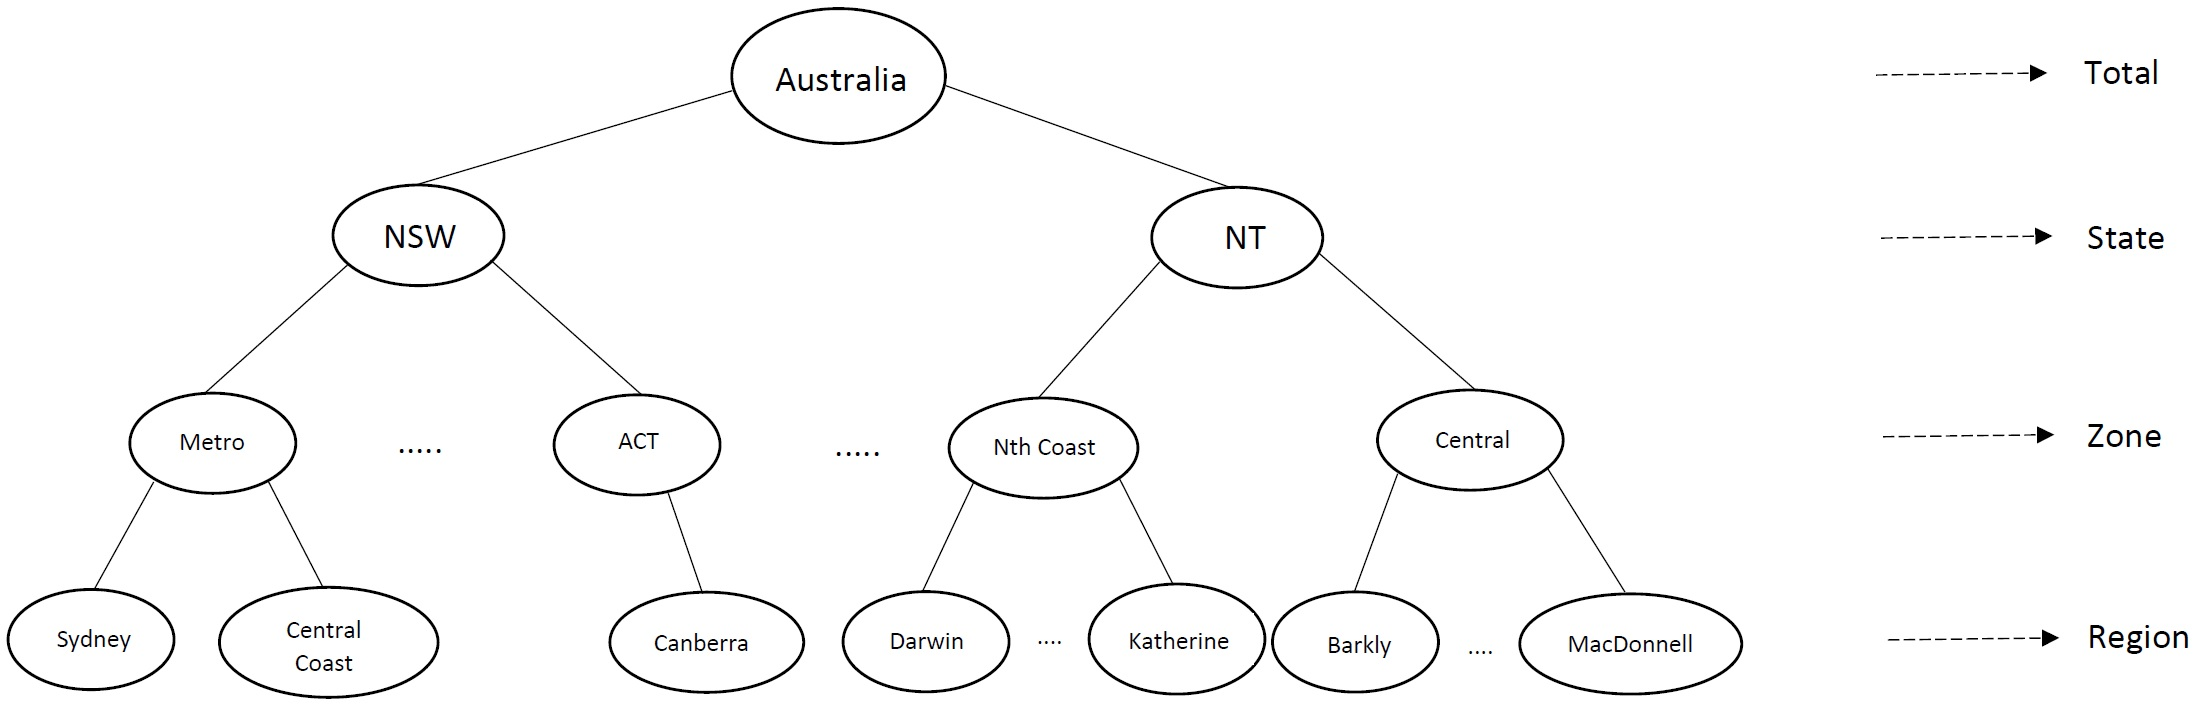
\includegraphics[width=450px,height=150px]{Paper-Figures/Australian_hierarchy_structure} 

}

\caption{Australia geographic hierarchical structure}\label{fig:Australiahierarchystructure}
\end{figure}

In this dataset we have three levels of geographic divisions in Australia. In the first level, Australia is divided into seven `States' including New South Wales (NSW), Victoria (VIC), Queensland (QLD), South Australia (SA), Western Australia (WA), Tasmania (TAS) and Northern Territory (NT). In the second and third levels, it is divided into 27 `Zones' and 76 `Regions' (for details about Australia geographic divisions see Figure \ref{fig:Australiahierarchystructure} and Table \ref{tab:Australiageographicaldivision}). For `Purpose' we have four groups: Holiday (Hol), Visiting friends and relatives (Vis), Business (Bus) and Other (Oth). Based on the geographic hierarchy and purpose grouping, we end up with 8 hierarchical levels with 555 series in total:

\begin{itemize}
\tightlist
\item
  Level 0 = Total for Australia
\item
  Level 1 = State totals
\item
  Level 2 = Zone totals
\item
  Level 3 = Region totals
\item
  Level 4 = Purpose totals
\item
  Level 5 = State \(\times\) Purpose totals
\item
  Level 6 = Zone \(\times\) Purpose totals
\item
  Level 7 = bottom level series
\end{itemize}

\begin{table}[!h]

\caption{\label{tab:Australiageographicalpurposedivision}Number of Australian domestic tourism series in each level of the hierarchy and group structure.}
\centering
\begin{tabular}{lrrr}
\toprule
Geographic division & \# series (geographic division) & \# series (purpose of travel) & Total\\
\midrule
Australia & 1 & 4 & 5\\
State & 7 & 28 & 35\\
Zone & 27 & 108 & 135\\
Region & 76 & 304 & 380\\
Total & 111 & 444 & 555\\
\bottomrule
\end{tabular}
\end{table}

We report the forecast results for all these hierarchical levels, as well as the average RMSE across all the levels of the hierarchy.

In the predictor matrix for the OLS forecasting model, we include a linear trend, 11 dummy variables, and 12 time series lags\footnote{Since the forecasting results are better with fewer lags, we use a linear trend and dummy seasonality variables and four lags in our linear model for 24-step-ahead model.}. This is intended to capture the monthly seasonality. In addition, before running the model, we partition the data into training and test sets, with the last 24 months (2 years) as our test set, and the rest as our training set.

\todo[inline]{Why not just use the four lag model from the start?}

\begin{table}[!h]

\caption{\label{tab:Tourismdataresulrolling}Mean(RMSE) for ETS, ARIMA and OLS with and without reconciliation - 1-step-ahead - Tourism dataset}
\centering
\begin{tabular}{lrrrrrr}
\toprule
\multicolumn{1}{c}{} & \multicolumn{3}{c}{Unreconciled} & \multicolumn{3}{c}{Reconciled} \\
\cmidrule(l{3pt}r{3pt}){2-4} \cmidrule(l{3pt}r{3pt}){5-7}
Level & ETS & ARIMA & OLS & ETS & ARIMA & OLS\\
\midrule
Level 0 & 1516.4 & 1445.5 & 1415.1 & 1533.6 & 1453.4 & 1454.4\\
Level 1 & 511.4 & 493.1 & 510.8 & 495.9 & 457.6 & 488.3\\
Level 2 & 214.8 & 219.0 & 224.5 & 209.2 & 207.5 & 212.4\\
Level 3 & 122.9 & 125.1 & 124.0 & 118.7 & 120.5 & 119.5\\
Level 4 & 676.0 & 709.2 & 694.5 & 668.3 & 679.7 & 678.5\\
Level 5 & 213.1 & 220.1 & 216.1 & 210.6 & 209.4 & 211.1\\
Level 6 & 97.5 & 102.4 & 101.0 & 96.4 & 99.8 & 98.6\\
Level 7 & 56.2 & 58.2 & 58.2 & 56.0 & 57.7 & 57.2\\
\bottomrule
\end{tabular}
\end{table}

\begin{table}[t]

\caption{\label{tab:TourismdataresultRMSE}Mean(RMSE) for ETS, ARIMA and OLS with and without reconciliation - 24-step-ahead - Tourism dataset}
\centering
\begin{tabular}{lrrrrrr}
\toprule
\multicolumn{1}{c}{} & \multicolumn{3}{c}{Unreconciled} & \multicolumn{3}{c}{Reconciled} \\
\cmidrule(l{3pt}r{3pt}){2-4} \cmidrule(l{3pt}r{3pt}){5-7}
Level & ETS & ARIMA & OLS & ETS & ARIMA & OLS\\
\midrule
Level 0 & 2238.6 & 3554.0 & 5050.3 & 2250.2 & 3179.4 & 4671.1\\
Level 1 & 593.6 & 570.1 & 900.1 & 553.8 & 626.3 & 903.0\\
Level 2 & 239.5 & 229.6 & 278.8 & 234.2 & 242.5 & 291.0\\
Level 3 & 132.6 & 129.4 & 142.8 & 126.7 & 129.4 & 146.3\\
Level 4 & 766.8 & 824.0 & 1307.0 & 795.5 & 958.2 & 1434.1\\
Level 5 & 226.7 & 241.2 & 298.2 & 222.5 & 236.9 & 308.4\\
Level 6 & 103.0 & 105.4 & 110.9 & 102.0 & 103.9 & 115.4\\
Level 7 & 59.1 & 58.8 & 60.9 & 58.5 & 58.7 & 62.6\\
\bottomrule
\end{tabular}
\end{table}

In Tables \ref{tab:Tourismdataresulrolling} and \ref{tab:TourismdataresultRMSE}, we show the average RMSE for the 1-month and 24-month forecasts. Methods include ETS, ARIMA and our proposed OLS forecasting model. In Table \ref{tab:Tourismdataresulrolling} we forecast 24 periods by computing 1-step-ahead ex post forecasts, rolling forward month by month. In Table \ref{tab:TourismdataresultRMSE} we generate 24-step-ahead ex ante forecasts. In these tables we show forecasts with and without reconciliation.

These results show that our proposed OLS forecasting model produces forecast accuracy similar to ETS and ARIMA, which are computationally heavy for many time series. Also they show the usefulness of the reconciliation in decreasing the average RMSE in all the three methods. Except for the total series, reconciliation can help in forecasting all the hierarchical levels.

In Figures \ref{fig:boxplotrollingtourism} and \ref{fig:boxplottourism} we display the error box plots for both reconciled and unreconciled forecasts using all three methods, for 1-step ahead and 24-steps ahead. In these figures we can visualize the error distributions across all the models, as well as usefulness of the reconciliation step in improving the forecasts. In particular, we see that by applying 1-step-ahead forecasts, the error densities are closer and more distributed around zero.

\begin{figure}

{\centering \includegraphics[width=1\linewidth]{hcf_files/figure-latex/boxplotrollingtourism-1} 

}

\caption{Box plot for forecast errors - Reconciled and unreconciled ETS, ARIMA and OLS in each hierarchical level for 1-step-ahead tourism demand.}\label{fig:boxplotrollingtourism}
\end{figure}

\begin{figure}

{\centering \includegraphics[width=1\linewidth]{hcf_files/figure-latex/boxplottourism-1} 

}

\caption{Box plot for forecast errors - Reconciled and unreconciled ETS, ARIMA and OLS in each hierarchical level for 24-step-ahead tourism demand}\label{fig:boxplottourism}
\end{figure}

Table \ref{tab:Tourismdatacomputationtime} compares the computation time of the three methods for 1-step-ahead and 24-step-ahead forecasting. We see that the OLS forecasting model is much faster compared to the other methods. Also, since reconciliation is a linear process, in all methods it is very fast and does not affect computation time significantly.

\begin{figure}

{\centering 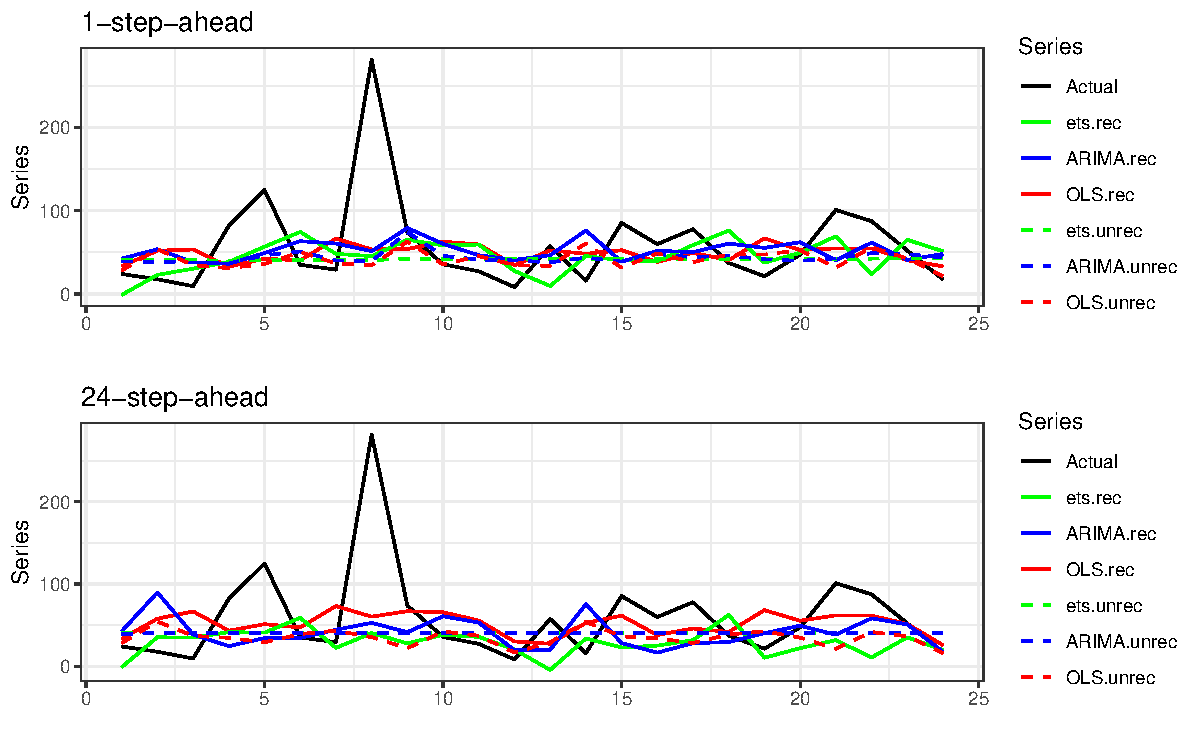
\includegraphics[width=1\linewidth]{hcf_files/figure-latex/forecstrolling24tourism-1} 

}

\caption{Comparing Actual test set, Reconciled and unreconciled ETS, ARIMA and OLS for BACBus bottom level series for 1-step-ahead and 24-step-ahead tourism demand.}\label{fig:forecstrolling24tourism}
\end{figure}

\begin{table}[t]

\caption{\label{tab:Tourismdatacomputationtime}Computation time (seconds) for ETS, ARIMA and OLS with and without reconciliation - 1- and 24-step-ahead - Tourism dataset}
\centering
\begin{tabular}{>{\centering\arraybackslash}p{3cm}>{\centering\arraybackslash}p{3cm}>{\centering\arraybackslash}p{3cm}cc}
\toprule
\multicolumn{1}{c}{} & \multicolumn{2}{c}{1-step-ahead} & \multicolumn{2}{c}{24-step-ahead} \\
\cmidrule(l{3pt}r{3pt}){2-3} \cmidrule(l{3pt}r{3pt}){4-5}
 & Unreconciled & Reconciled & Unreconciled & Reconciled\\
\midrule
ETS & 10924.57 & 10924.60 & 407.10 & 407.15\\
ARIMA & 31146.38 & 31146.52 & 1116.15 & 1116.19\\
OLS & 48.40 & 48.31 & 16.66 & 16.85\\
\bottomrule
\end{tabular}
\end{table}

Now since we are using a linear model for forecasting, we can easily include information about the timing of Easter to check its effect on forecasting results. We also add this information on ARIMA models and compare with the OLS forecasting model. In Tables \ref{tab:easterroolingRMSE} and \ref{tab:easterRMSE}, we display the average RMSE of ARIMA and OLS including the easter information, ARIMAX and OLSX, across different levels with and without reconciliation. These tables are for 1-step-ahead and 24-step-ahead forecasts. Figure \ref{fig:forecstrolling24tourism} shows the 1-step-ahead and 24-step-ahead forecast results for one of the bottom level series, BACBus (Geelong/Business). In these plots we have both reconciled (solid lines) and unreconciled (dashed lines) forecasts and we see that the reconciliation step improves the forecasts in this series. We also see that the OLS model forecast accuracy is similar to the other two methods. These results show that adding this external data does not change the forecasting results significantly. However in different cases, trying different external data can be helpful in improving the forecasting results.

\begin{table}[t]

\caption{\label{tab:easterroolingRMSE}Mean(RMSE) for ETS, ARIMA and OLS with and without reconciliation - 1-step-ahead - Tourism dataset}
\centering
\begin{tabular}{lrrrrrrrr}
\toprule
\multicolumn{1}{c}{} & \multicolumn{4}{c}{Unreconciled} & \multicolumn{4}{c}{Reconciled} \\
\cmidrule(l{3pt}r{3pt}){2-5} \cmidrule(l{3pt}r{3pt}){6-9}
Level & ARIMA & OLS & ARIMAX & OLSX & ARIMA & OLS & ARIMAX & OLSX\\
\midrule
Level 0 & 1445.5 & 1415.1 & 1565.0 & 1444.5 & 1453.4 & 1454.4 & 1546.5 & 1487.2\\
Level 1 & 493.1 & 510.8 & 500.7 & 514.3 & 457.6 & 488.3 & 472.0 & 492.7\\
Level 2 & 219.0 & 224.5 & 220.9 & 225.8 & 207.5 & 212.4 & 210.5 & 213.5\\
Level 3 & 125.1 & 124.0 & 125.8 & 123.7 & 120.5 & 119.5 & 121.0 & 119.4\\
Level 4 & 709.2 & 694.5 & 702.8 & 680.6 & 679.7 & 678.5 & 682.9 & 662.4\\
Level 5 & 220.1 & 216.1 & 222.1 & 215.1 & 209.4 & 211.1 & 211.5 & 209.6\\
Level 6 & 102.4 & 101.0 & 103.0 & 100.9 & 99.8 & 98.6 & 100.5 & 98.5\\
Level 7 & 58.2 & 58.2 & 58.6 & 58.1 & 57.7 & 57.2 & 58.0 & 57.2\\
\bottomrule
\end{tabular}
\end{table}

\begin{table}[t]

\caption{\label{tab:easterRMSE}Mean(RMSE) for ETS, ARIMA and OLS with and without reconciliation - 24-step-ahead - Tourism dataset}
\centering
\begin{tabular}{lrrrrrrrr}
\toprule
\multicolumn{1}{c}{} & \multicolumn{4}{c}{Unreconciled} & \multicolumn{4}{c}{Reconciled} \\
\cmidrule(l{3pt}r{3pt}){2-5} \cmidrule(l{3pt}r{3pt}){6-9}
Level & ARIMA & OLS & ARIMAX & OLSX & ARIMA & OLS & ARIMAX & OLSX\\
\midrule
Level 0 & 3554.0 & 5050.3 & 3528.1 & 5032.4 & 3179.4 & 4671.1 & 3114.4 & 4678.0\\
Level 1 & 570.1 & 900.1 & 509.8 & 910.7 & 626.3 & 903.0 & 603.7 & 907.3\\
Level 2 & 229.6 & 278.8 & 235.1 & 280.1 & 242.5 & 291.0 & 243.8 & 291.6\\
Level 3 & 129.4 & 142.8 & 129.4 & 143.7 & 129.4 & 146.3 & 129.6 & 147.2\\
Level 4 & 824.0 & 1307.0 & 811.1 & 1324.7 & 958.2 & 1434.1 & 930.7 & 1444.8\\
Level 5 & 241.2 & 298.2 & 232.9 & 304.6 & 236.9 & 308.4 & 229.6 & 313.5\\
Level 6 & 105.4 & 110.9 & 104.7 & 111.9 & 103.9 & 115.4 & 104.5 & 116.3\\
Level 7 & 58.8 & 60.9 & 59.2 & 61.4 & 58.7 & 62.6 & 59.0 & 63.1\\
\bottomrule
\end{tabular}
\end{table}

\todo[inline]{I can't see much point including these Easter results.}

\FloatBarrier

\hypertarget{wikipedia-pageviews}{%
\subsection{Wikipedia pageviews}\label{wikipedia-pageviews}}

The second dataset consists of one year of daily data (2016-06-01 to 2017-06-29) on Wikipedia pageviews for the most popular social networks articles \autocite{ashouri2018}. This dataset is noisier compared with the Australian monthly tourism data and forecasting its series is more challenging. It has a grouped structure, with grouping attributes: `Agent': Spider, User, `Access': Desktop, Mobile app, Mobile web, `Language': en (English), de (German), es (Spanish), zh (Chinese) and `Purpose': Blogging related, Business, Gaming, General purpose, Life style, Photo sharing, Reunion, Travel, Video (check Table \ref{tab:wikipediagroupingstructure}). We display the group structure in Table \ref{tab:wikipediagroupingstructure} and Figure \ref{fig:wikigroupstructure}. In Figure \ref{fig:wikigroupstructure} we use one possible hierarchy for this dataset, but the order of the hierarchy can be switched.
The final dataset includes 913 time series, each with length 394. The group structure and different levels include:

\begin{itemize}
\tightlist
\item
  Level 0 = Total
\item
  Level 1 = Agent
\item
  Level 2 = Access
\item
  Level 3 = Language
\item
  Level 4 = Purpose
\item
  Level 5 = bottom level series
\end{itemize}

For this daily dataset, in the OLS forecasting model we include in the predictor matrix a linear trend, 6 seasonal dummies and 7 lags. We partitioned the data into two parts training and test sets. We used the last 28 days for our test set and the rest for the training set.

\begin{table}[t]

\caption{\label{tab:wikipediagroupingstructure}Social networking Wikipedia article grouping structure}
\centering
\begin{tabular}{crcr}
\toprule
Series & Name & Series & Name\\
\midrule
Total &  & Language & \\
1 & Social Network & 10 & zh (Chinese)\\
Agent &  & Purpose & \\
2 & Spider & 11 & Blogging related\\
3 & User & 12 & Business\\
Access &  & 13 & Gaming\\
4 & Desktop & 14 & General purpose\\
5 & Mobile app & 15 & Life style\\
6 & Mobile web & 16 & Photo sharing\\
Language &  & 17 & Reunion\\
7 & en (English) & 18 & Travel\\
8 & de (German) & 19 & Video\\
9 & es (Spanish) &  & \\
\bottomrule
\end{tabular}
\end{table}

\begin{figure}

{\centering 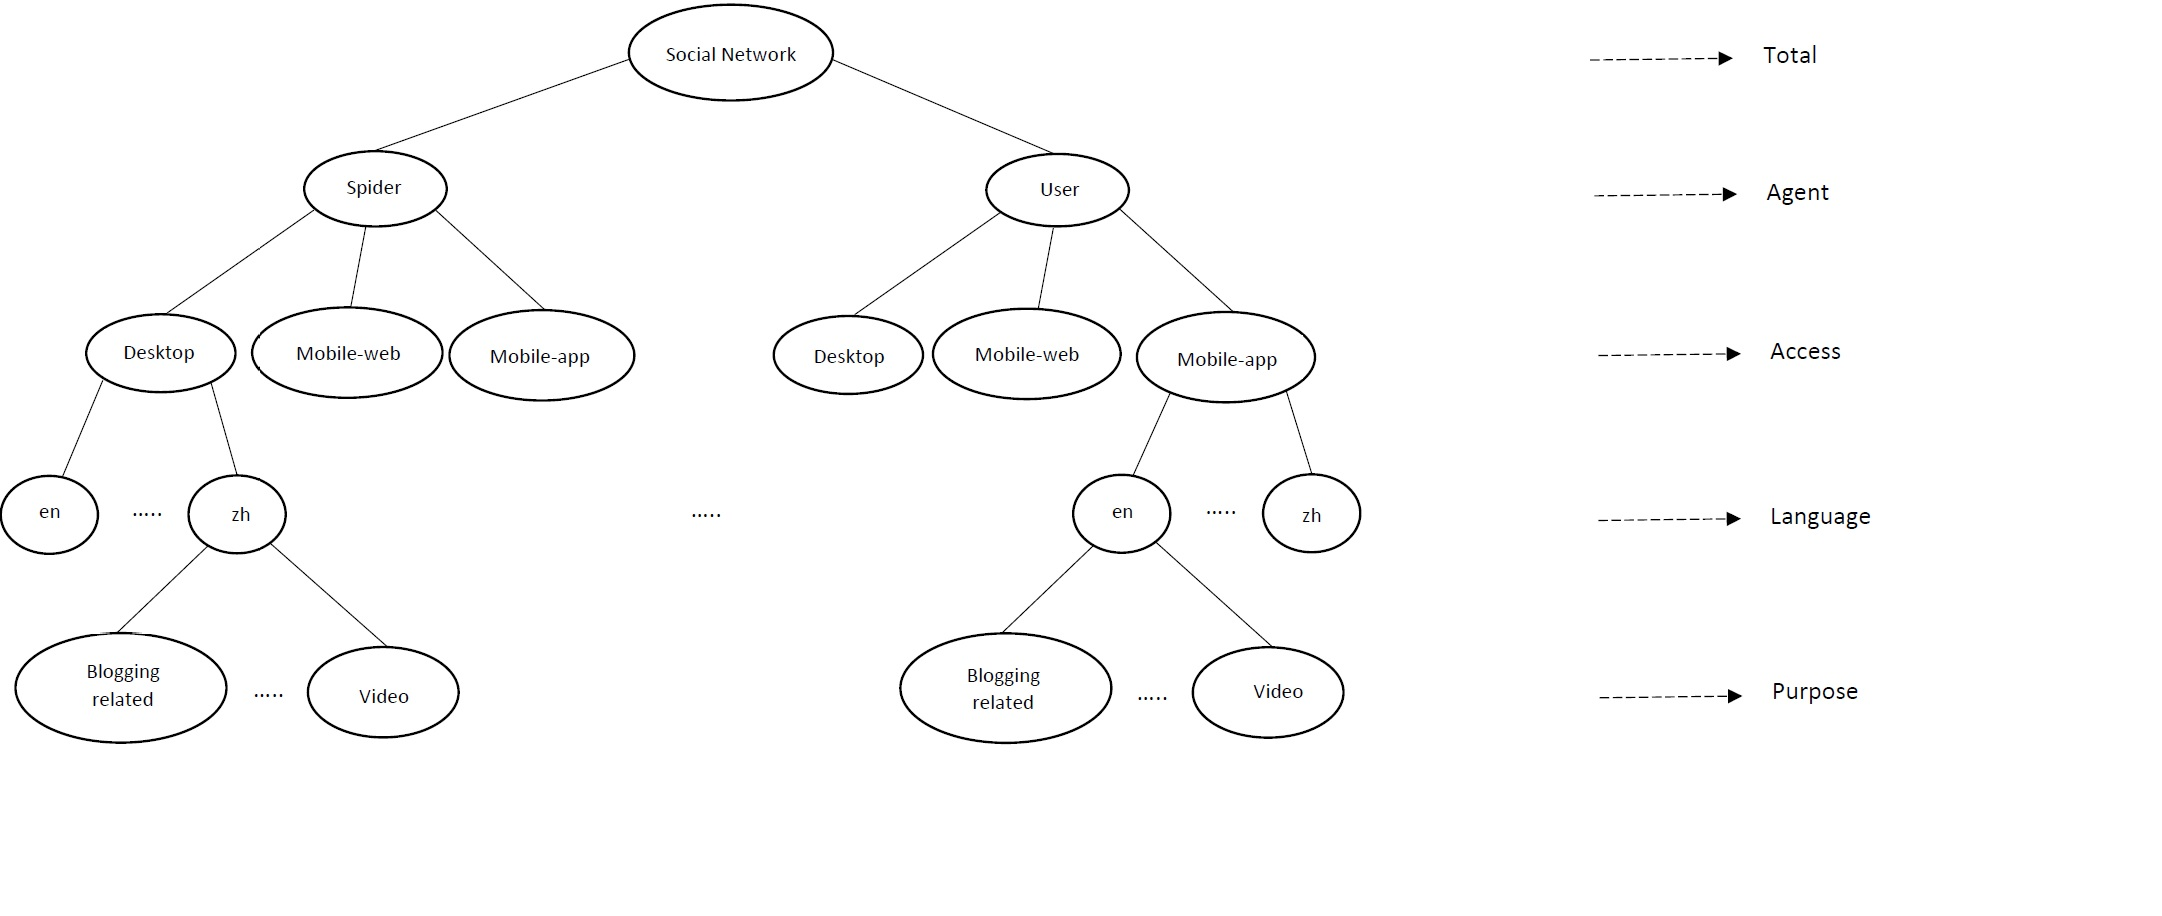
\includegraphics[width=500px,height=250px]{Paper-Figures/Wiki_group_structure} 

}

\caption{One of the possible hierarchical structures for Wikipedia pageview dataset}\label{fig:wikigroupstructure}
\end{figure}

Table \ref{tab:wikipediadataresulrolling}, \ref{tab:wikipediadataresultRMSE} and \ref{tab:wikipediadatacomputationtime} represent the RMSE results and computation time. Although these time series are noisier, still we get acceptable results for the OLS forecasting model compared with ETS and ARIMA. In this case, we get similar results with and without the reconciliation step in the forecasted errors.

Figures \ref{fig:boxplotrollingwiki} and \ref{fig:boxplotwiki} display the forecast error box plot. These plots are for 1-step-ahead and 28-step-ahead forecasts in each level of grouping. Further, we can see that the error distribution is almost similar in all levels across the different methods. The only exception is the Total series, where ETS performs significantly better than ARIMA and OLS. We also note that the reconciliation is less effective.

\begin{table}[t]

\caption{\label{tab:wikipediadataresulrolling}Mean(RMSE) for ETS, ARIMA and OLS with and without reconciliation - 1-step-ahead - Wikipedia dataset}
\centering
\begin{tabular}{ccccccc}
\toprule
\multicolumn{1}{c}{} & \multicolumn{6}{c}{Mean(RMSE)} \\
\cmidrule(l{3pt}r{3pt}){2-7}
\multicolumn{1}{c}{} & \multicolumn{3}{c}{Unreconciled} & \multicolumn{3}{c}{Reconciled} \\
\cmidrule(l{3pt}r{3pt}){2-4} \cmidrule(l{3pt}r{3pt}){5-7}
 & ETS & ARIMA & OLS & ETS & ARIMA & OLS\\
\midrule
Level 0 & 10773.66 & 15060.65 & 15748.18 & 11014.73 & 14276.47 & 15270.23\\
Level 1 & 8272.92 & 10196.34 & 10623.85 & 7736.88 & 9904.12 & 10673.98\\
Level 2 & 6524.72 & 6705.03 & 6979.58 & 6257.44 & 7142.49 & 7285.97\\
Level 3 & 4870.08 & 6333.02 & 7150.13 & 4981.91 & 6369.98 & 7106.11\\
Level 4 & 5233.50 & 4659.53 & 4675.18 & 5001.40 & 4586.53 & 4650.26\\
Level 5 & 358.90 & 238.97 & 254.98 & 362.25 & 241.60 & 256.11\\
\bottomrule
\end{tabular}
\end{table}

\begin{figure}

{\centering 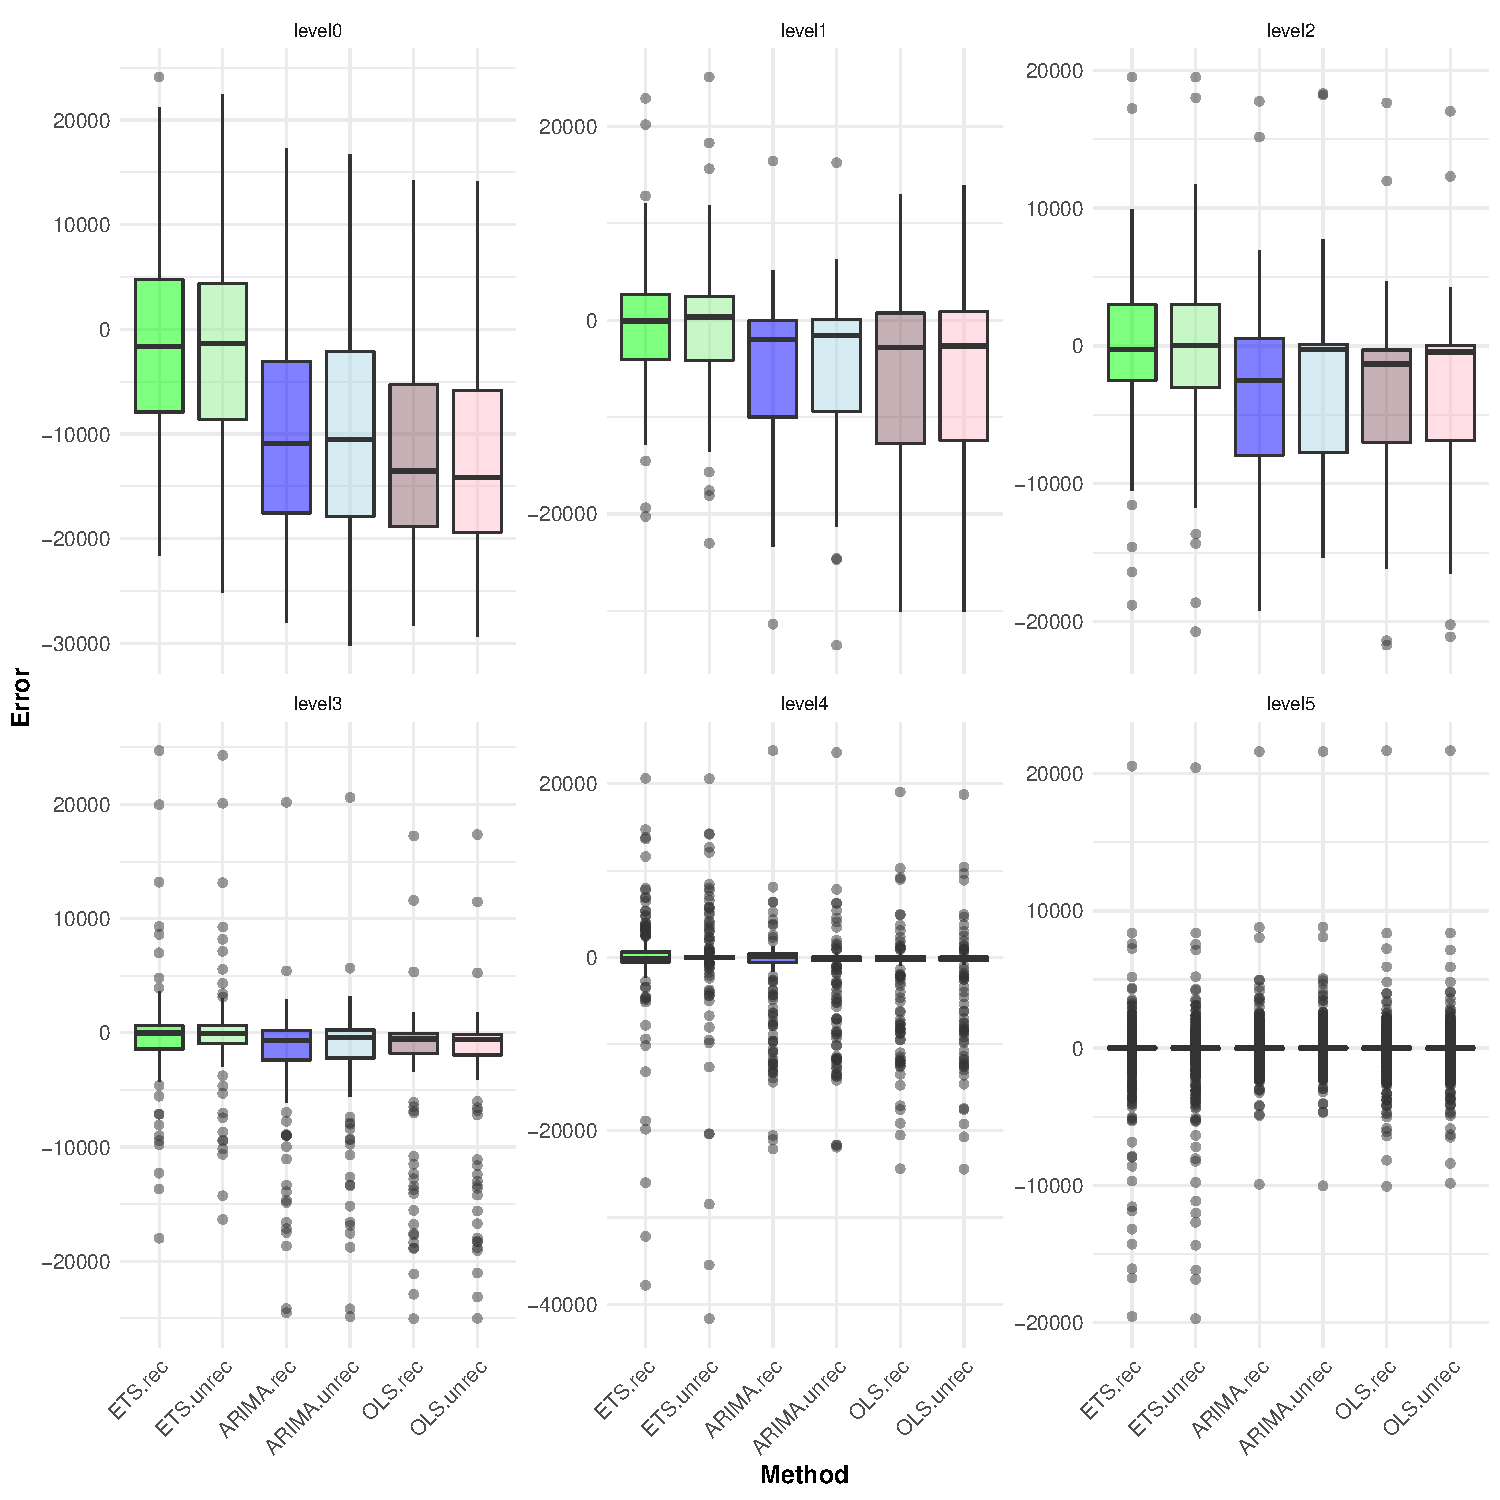
\includegraphics[width=450px,height=300px]{Paper-Figures/results_Wikipedia/boxplot_1} 

}

\caption{Box plot for forecast errors -  Reconciled and unreconciled ETS, ARIMA and OLS in each hierarchical level for 1-step-ahead Wikipedia pageviews}\label{fig:boxplotrollingwiki}
\end{figure}

\begin{table}[t]

\caption{\label{tab:wikipediadataresultRMSE}Mean(RMSE) for ETS, ARIMA and OLS with and without reconciliation - 28-step-ahead - Wikipedia dataset}
\centering
\begin{tabular}{ccccccc}
\toprule
\multicolumn{1}{c}{} & \multicolumn{6}{c}{Mean(RMSE)} \\
\cmidrule(l{3pt}r{3pt}){2-7}
\multicolumn{1}{c}{} & \multicolumn{3}{c}{Unreconciled} & \multicolumn{3}{c}{Reconciled} \\
\cmidrule(l{3pt}r{3pt}){2-4} \cmidrule(l{3pt}r{3pt}){5-7}
 & ETS & ARIMA & OLS & ETS & ARIMA & OLS\\
\midrule
Level 0 & 14846.93 & 24298.84 & 29840.58 & 14999.18 & 24649.91 & 29665.70\\
Level 1 & 13608.73 & 17277.01 & 21165.30 & 12240.30 & 16810.45 & 21048.06\\
Level 2 & 7117.43 & 10731.97 & 12678.89 & 7523.43 & 11068.81 & 12811.18\\
Level 3 & 6475.90 & 9580.38 & 12056.62 & 6509.03 & 9799.11 & 12112.46\\
Level 4 & 5302.74 & 8611.25 & 8451.09 & 5307.34 & 8239.77 & 8460.35\\
Level 5 & 435.64 & 390.05 & 389.41 & 437.67 & 391.22 & 390.97\\
\bottomrule
\end{tabular}
\end{table}

\begin{figure}

{\centering 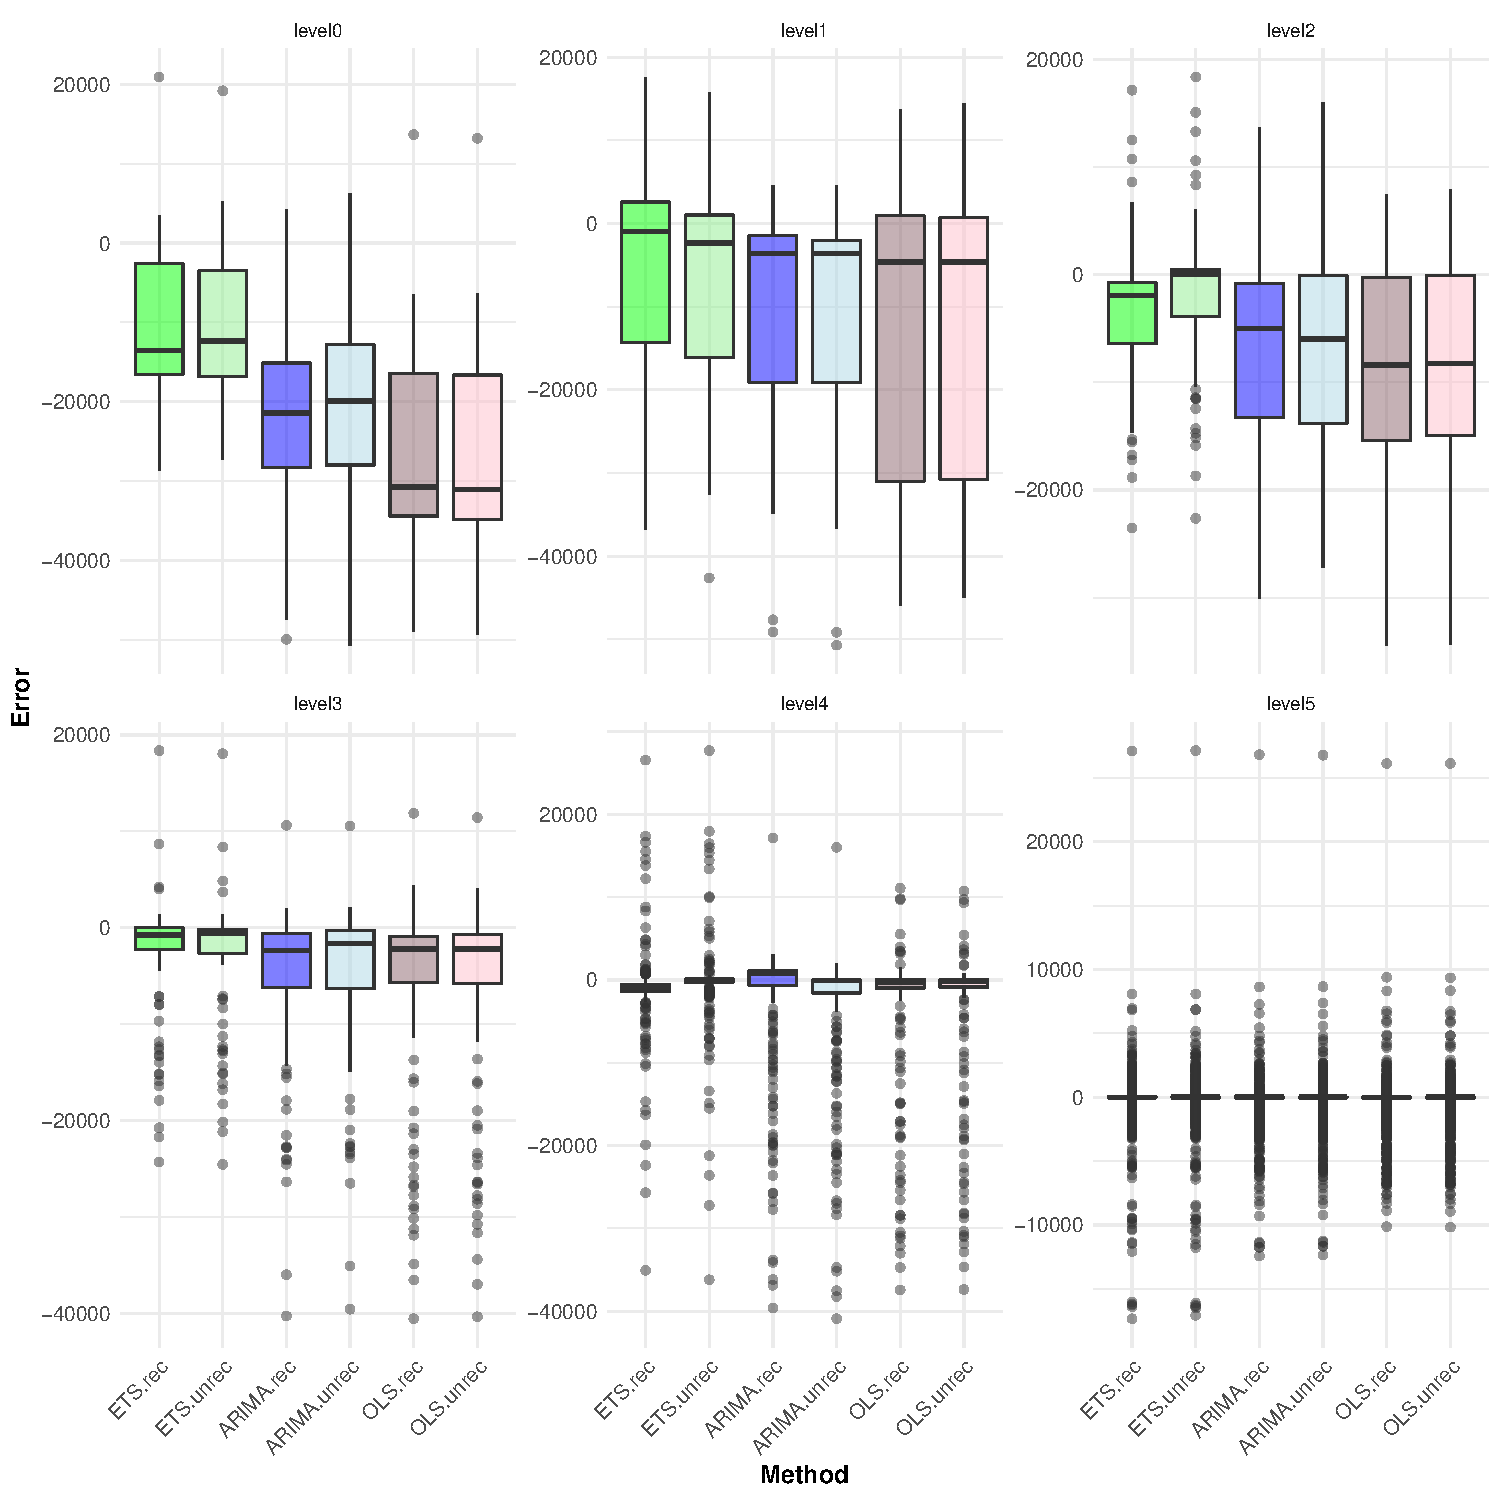
\includegraphics[width=450px,height=300px]{Paper-Figures/results_Wikipedia/boxplot_28} 

}

\caption{Box plot for forecast errors -  Reconciled and unreconciled ETS, ARIMA and OLS in each hierarchical level for 28-step-ahead Wikipedia pageviews}\label{fig:boxplotwiki}
\end{figure}

In Figure \ref{fig:forecstrolling28wiki}, we display results for one of the bottom level series, desktopusenPho (desktop-user-english-photo sharing). The plot shows 1-step-ahead and 28-step-ahead forecast results for ETS, ARIMA and OLS, with (solid lines) and without (dashed lines) applying reconciliation. We see that the OLS forecasting model performs close to the other two methods, and reconciliation improves the forecasts.

\begin{figure}

{\centering 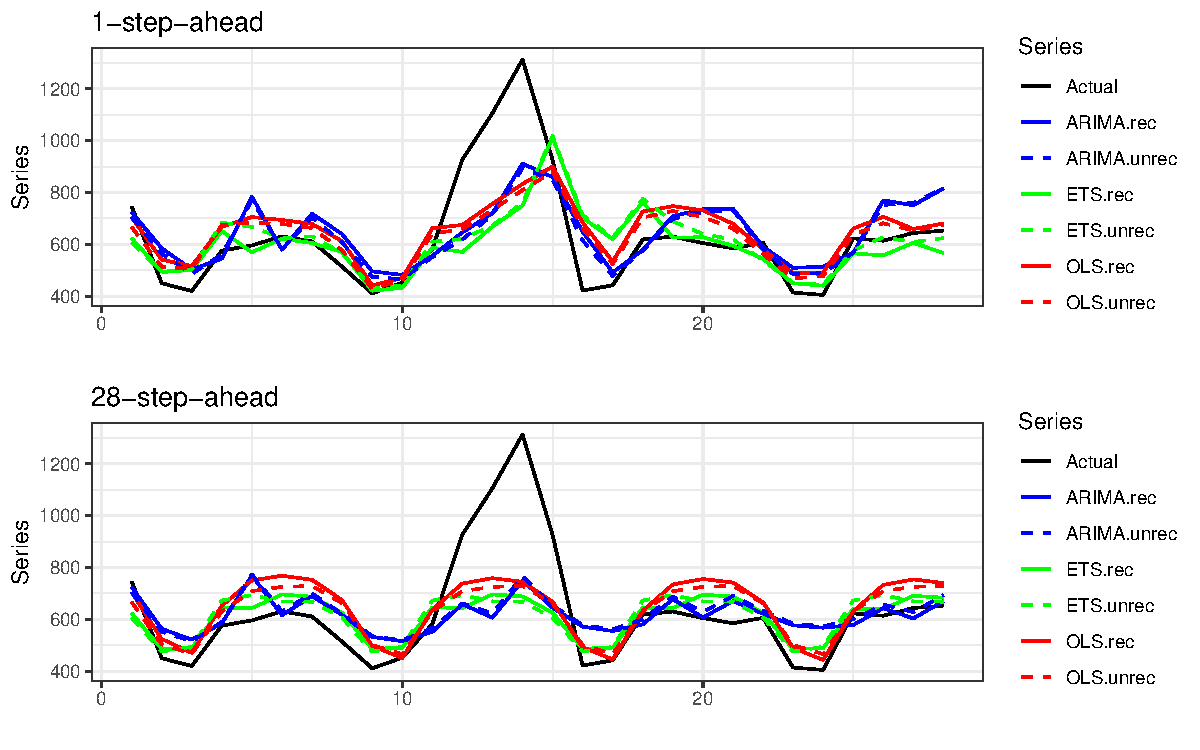
\includegraphics[width=400px,height=300px]{hcf_files/figure-latex/forecstrolling28wiki-1} 

}

\caption{Comparing Actual test set, Reconciled and unreconciled ETS, ARIMA and OLS for desktopusenPho (desktop-user-english-photo sharing)  bottom level series- 1- and 28-step-ahead Wikipedia pageviews}\label{fig:forecstrolling28wiki}
\end{figure}

Lastly, Table \ref{tab:wikipediadatacomputationtime} presents the computation times for all three methods. ETS and ARIMA are clearly much more computationally heavy compared with OLS. As in the Australian tourism dataset, running reconciliation does not have much effect on computation time.

\begin{table}[t]

\caption{\label{tab:wikipediadatacomputationtime}Computation time (seconds) for ETS, ARIMA and OLS with and without reconciliation - 1- and 28-step-ahead - Wikipedia dataset}
\centering
\begin{tabular}{>{\centering\arraybackslash}p{3cm}>{\centering\arraybackslash}p{3cm}>{\centering\arraybackslash}p{3cm}cc}
\toprule
\multicolumn{1}{c}{} & \multicolumn{4}{c}{Computation time (secs)} \\
\cmidrule(l{3pt}r{3pt}){2-5}
\multicolumn{1}{c}{} & \multicolumn{2}{c}{1-step-ahead} & \multicolumn{2}{c}{28-step-ahead} \\
\cmidrule(l{3pt}r{3pt}){2-3} \cmidrule(l{3pt}r{3pt}){4-5}
 & Unreconciled & Reconciled & Unreconciled & Reconciled\\
\midrule
ETS & 13963.93 & 13963.96 & 450.89 & 450.92\\
ARIMA & 10327.02 & 10327.15 & 670.40 & 670.44\\
OLS & 82.55 & 82.62 & 35.39 & 35.43\\
\bottomrule
\end{tabular}
\end{table}

\hypertarget{conclusion}{%
\section{Conclusion}\label{conclusion}}

We proposed a single-step linear approach to forecast hierarchical or grouped time series in a much faster way, but with accuracy that nearly matches that of forecast methods such as ETS and ARIMA. This is especially useful in large collections of time series, as is typical in hierarchical and grouped structures. Although ETS and ARIMA are good in terms of forecasting power and accuracy, they can be computationally heavy when facing large collections of time series in the hierarchy. Adding another faster option for calculating base forecasts was our purpose in this research. Here we suggest a linear model, OLS, instead of ETS and ARIMA which is not computationally intensive. We also showed that OLS can compete ETS and ARIMA in terms of forecasting accuracy level. We also note that OLS has the additional practice feature in handling missing data while ETS and ARIMA requires imputation. One more important feature of our model is the ability to easily include external information such as holiday dummies or other external series. In addition to the computation adjustment, our proposed approach forecasts hierarchical time series in a parsimonious single step whereas other available methods all forecast in two-steps.

\hypertarget{acknowledgements}{%
\section{Acknowledgements}\label{acknowledgements}}

The first and third authors of this research were partially funded by Ministry of Science and Technology (MOST), Taiwan {[}Grant 106-2420-H-007-019{]}.

\printbibliography

\end{document}
